\documentclass{article}

\usepackage[margin=2cm]{geometry}
\usepackage{amsmath,amsfonts}
\usepackage{mathtools}
\usepackage{graphicx}
\usepackage{caption}
\usepackage{subcaption}
\usepackage{color}
\newcommand\fb[1]{\textcolor{blue}{FB: #1}}
\newcommand\ah[1]{\textcolor{red}{AH: #1}}
\usepackage{subfiles}

% -------- MACROS ----------%


\newcommand{\xmu}[2]{x_{#1_#2}^{#2}(t)}
\newcommand{\xmudash}[2]{x_{#1_#2}^{#2}(t')}
\newcommand{\payoff}[2]{P^{#2}_{#1_#2, #1_{-#2}}}

\newcommand{\dxmu}[1]{\dot{x}_{#1_\mu}^{\mu} (t)}
\newcommand{\hxmu}[1]{\hat{x}_{#1_\mu}^{\mu} (t)}
\newcommand{\hxnu}[1]{\hat{x}_{#1_\nu}^{\nu} (t)}
\newcommand{\hxmudash}[1]{\hat{x}_{#1_\mu}^{\mu} (t')}
\newcommand{\hxnudash}[1]{\hat{x}_{#1_\nu}^{\nu} (t')}

\newcommand{\txmu}[2]{\tilde{x}_{#1_#2}^{#2}(t)}
\newcommand{\dtxmu}[2]{\dot{\tilde{x}}_{#1_#2}^{#2}(t)}
\newcommand{\tpayoff}[2]{\tilde{P}^{#2}_{#1_#2, #1_{-#2}}}
\newcommand{\talpha}{\tilde{\alpha}}
\newcommand{\ttau}{\tilde{\tau}}
\newcommand{\htau}{\hat{\tau}}
\newcommand{\xfixed}{x_\infty}
\newcommand{\ezerof}{\eta_{0, \infty}}
\newcommand{\eonef}{\eta_{1, \infty}}

\newcommand{\xpert}{\hat{x}(t)}
\newcommand{\xpertdash}{\hat{x}(t')}
\newcommand{\ezeropert}{\hat{\eta}_0(t)}
\newcommand{\eonepert}{\hat{\eta}_1(t)}

\newcommand{\eom}{\frac{\dxmu{i}}{\xmu{i}{\mu}} - \alpha \ttau \left ( \sum_{i_{-\mu}} \payoff{i}{\mu} \prod_{\kappa \neq \mu} \xmu{i}{\kappa} \right ) + \\ \alpha \htau \left ( \frac{1}{\sqrt{N}} \sum_{i_\mu i_{-\mu}} \xmu{i}{\mu} \payoff{i}{\mu} \prod_{\kappa \neq \mu} \xmu{i}{\kappa} \right ) - \talpha \rho^{\mu}_{i}(t)}
% ---- END MACROS ------- %

% ----- PREAMBLE FOR CODE ---- %

    \usepackage[breakable]{tcolorbox}
    \usepackage{parskip} % Stop auto-indenting (to mimic markdown behaviour)
    
    \usepackage{iftex}
    \ifPDFTeX
    	\usepackage[T1]{fontenc}
    	\usepackage{mathpazo}
    \else
    	\usepackage{fontspec}
    \fi

    % Basic figure setup, for now with no caption control since it's done
    % automatically by Pandoc (which extracts ![](path) syntax from Markdown).
    \usepackage{graphicx}
    % Maintain compatibility with old templates. Remove in nbconvert 6.0
    \let\Oldincludegraphics\includegraphics
    % Ensure that by default, figures have no caption (until we provide a
    % proper Figure object with a Caption API and a way to capture that
    % in the conversion process - todo).
    \usepackage{caption}
    \DeclareCaptionFormat{nocaption}{}
    \captionsetup{format=nocaption,aboveskip=0pt,belowskip=0pt}

    \usepackage{float}
    \floatplacement{figure}{H} % forces figures to be placed at the correct location
    \usepackage{xcolor} % Allow colors to be defined
    \usepackage{enumerate} % Needed for markdown enumerations to work
    \usepackage{geometry} % Used to adjust the document margins
    \usepackage{amsmath} % Equations
    \usepackage{amssymb} % Equations
    \usepackage{textcomp} % defines textquotesingle
    % Hack from http://tex.stackexchange.com/a/47451/13684:
    \AtBeginDocument{%
        \def\PYZsq{\textquotesingle}% Upright quotes in Pygmentized code
    }
    \usepackage{upquote} % Upright quotes for verbatim code
    \usepackage{eurosym} % defines \euro
    \usepackage[mathletters]{ucs} % Extended unicode (utf-8) support
    \usepackage{fancyvrb} % verbatim replacement that allows latex
    \usepackage{grffile} % extends the file name processing of package graphics 
                         % to support a larger range
    \makeatletter % fix for old versions of grffile with XeLaTeX
    \@ifpackagelater{grffile}{2019/11/01}
    {
      % Do nothing on new versions
    }
    {
      \def\Gread@@xetex#1{%
        \IfFileExists{"\Gin@base".bb}%
        {\Gread@eps{\Gin@base.bb}}%
        {\Gread@@xetex@aux#1}%
      }
    }
    \makeatother
    \usepackage[Export]{adjustbox} % Used to constrain images to a maximum size
    \adjustboxset{max size={0.9\linewidth}{0.9\paperheight}}

    % The hyperref package gives us a pdf with properly built
    % internal navigation ('pdf bookmarks' for the table of contents,
    % internal cross-reference links, web links for URLs, etc.)
    \usepackage{hyperref}
    % The default LaTeX title has an obnoxious amount of whitespace. By default,
    % titling removes some of it. It also provides customization options.
    \usepackage{titling}
    \usepackage{longtable} % longtable support required by pandoc >1.10
    \usepackage{booktabs}  % table support for pandoc > 1.12.2
    \usepackage[inline]{enumitem} % IRkernel/repr support (it uses the enumerate* environment)
    \usepackage[normalem]{ulem} % ulem is needed to support strikethroughs (\sout)
                                % normalem makes italics be italics, not underlines
    \usepackage{mathrsfs}
    

    
    % Colors for the hyperref package
    \definecolor{urlcolor}{rgb}{0,.145,.698}
    \definecolor{linkcolor}{rgb}{.71,0.21,0.01}
    \definecolor{citecolor}{rgb}{.12,.54,.11}

    % ANSI colors
    \definecolor{ansi-black}{HTML}{3E424D}
    \definecolor{ansi-black-intense}{HTML}{282C36}
    \definecolor{ansi-red}{HTML}{E75C58}
    \definecolor{ansi-red-intense}{HTML}{B22B31}
    \definecolor{ansi-green}{HTML}{00A250}
    \definecolor{ansi-green-intense}{HTML}{007427}
    \definecolor{ansi-yellow}{HTML}{DDB62B}
    \definecolor{ansi-yellow-intense}{HTML}{B27D12}
    \definecolor{ansi-blue}{HTML}{208FFB}
    \definecolor{ansi-blue-intense}{HTML}{0065CA}
    \definecolor{ansi-magenta}{HTML}{D160C4}
    \definecolor{ansi-magenta-intense}{HTML}{A03196}
    \definecolor{ansi-cyan}{HTML}{60C6C8}
    \definecolor{ansi-cyan-intense}{HTML}{258F8F}
    \definecolor{ansi-white}{HTML}{C5C1B4}
    \definecolor{ansi-white-intense}{HTML}{A1A6B2}
    \definecolor{ansi-default-inverse-fg}{HTML}{FFFFFF}
    \definecolor{ansi-default-inverse-bg}{HTML}{000000}

    % common color for the border for error outputs.
    \definecolor{outerrorbackground}{HTML}{FFDFDF}

    % commands and environments needed by pandoc snippets
    % extracted from the output of `pandoc -s`
    \providecommand{\tightlist}{%
      \setlength{\itemsep}{0pt}\setlength{\parskip}{0pt}}
    \DefineVerbatimEnvironment{Highlighting}{Verbatim}{commandchars=\\\{\}}
    % Add ',fontsize=\small' for more characters per line
    \newenvironment{Shaded}{}{}
    \newcommand{\KeywordTok}[1]{\textcolor[rgb]{0.00,0.44,0.13}{\textbf{{#1}}}}
    \newcommand{\DataTypeTok}[1]{\textcolor[rgb]{0.56,0.13,0.00}{{#1}}}
    \newcommand{\DecValTok}[1]{\textcolor[rgb]{0.25,0.63,0.44}{{#1}}}
    \newcommand{\BaseNTok}[1]{\textcolor[rgb]{0.25,0.63,0.44}{{#1}}}
    \newcommand{\FloatTok}[1]{\textcolor[rgb]{0.25,0.63,0.44}{{#1}}}
    \newcommand{\CharTok}[1]{\textcolor[rgb]{0.25,0.44,0.63}{{#1}}}
    \newcommand{\StringTok}[1]{\textcolor[rgb]{0.25,0.44,0.63}{{#1}}}
    \newcommand{\CommentTok}[1]{\textcolor[rgb]{0.38,0.63,0.69}{\textit{{#1}}}}
    \newcommand{\OtherTok}[1]{\textcolor[rgb]{0.00,0.44,0.13}{{#1}}}
    \newcommand{\AlertTok}[1]{\textcolor[rgb]{1.00,0.00,0.00}{\textbf{{#1}}}}
    \newcommand{\FunctionTok}[1]{\textcolor[rgb]{0.02,0.16,0.49}{{#1}}}
    \newcommand{\RegionMarkerTok}[1]{{#1}}
    \newcommand{\ErrorTok}[1]{\textcolor[rgb]{1.00,0.00,0.00}{\textbf{{#1}}}}
    \newcommand{\NormalTok}[1]{{#1}}
    
    % Additional commands for more recent versions of Pandoc
    \newcommand{\ConstantTok}[1]{\textcolor[rgb]{0.53,0.00,0.00}{{#1}}}
    \newcommand{\SpecialCharTok}[1]{\textcolor[rgb]{0.25,0.44,0.63}{{#1}}}
    \newcommand{\VerbatimStringTok}[1]{\textcolor[rgb]{0.25,0.44,0.63}{{#1}}}
    \newcommand{\SpecialStringTok}[1]{\textcolor[rgb]{0.73,0.40,0.53}{{#1}}}
    \newcommand{\ImportTok}[1]{{#1}}
    \newcommand{\DocumentationTok}[1]{\textcolor[rgb]{0.73,0.13,0.13}{\textit{{#1}}}}
    \newcommand{\AnnotationTok}[1]{\textcolor[rgb]{0.38,0.63,0.69}{\textbf{\textit{{#1}}}}}
    \newcommand{\CommentVarTok}[1]{\textcolor[rgb]{0.38,0.63,0.69}{\textbf{\textit{{#1}}}}}
    \newcommand{\VariableTok}[1]{\textcolor[rgb]{0.10,0.09,0.49}{{#1}}}
    \newcommand{\ControlFlowTok}[1]{\textcolor[rgb]{0.00,0.44,0.13}{\textbf{{#1}}}}
    \newcommand{\OperatorTok}[1]{\textcolor[rgb]{0.40,0.40,0.40}{{#1}}}
    \newcommand{\BuiltInTok}[1]{{#1}}
    \newcommand{\ExtensionTok}[1]{{#1}}
    \newcommand{\PreprocessorTok}[1]{\textcolor[rgb]{0.74,0.48,0.00}{{#1}}}
    \newcommand{\AttributeTok}[1]{\textcolor[rgb]{0.49,0.56,0.16}{{#1}}}
    \newcommand{\InformationTok}[1]{\textcolor[rgb]{0.38,0.63,0.69}{\textbf{\textit{{#1}}}}}
    \newcommand{\WarningTok}[1]{\textcolor[rgb]{0.38,0.63,0.69}{\textbf{\textit{{#1}}}}}
    
    
    % Define a nice break command that doesn't care if a line doesn't already
    % exist.
    \def\br{\hspace*{\fill} \\* }
    % Math Jax compatibility definitions
    \def\gt{>}
    \def\lt{<}
    \let\Oldtex\TeX
    \let\Oldlatex\LaTeX
    \renewcommand{\TeX}{\textrm{\Oldtex}}
    \renewcommand{\LaTeX}{\textrm{\Oldlatex}}
    % Document parameters
    % Document title
    \title{pPlayerJulia}
    
    
    
    
    
% Pygments definitions
\makeatletter
\def\PY@reset{\let\PY@it=\relax \let\PY@bf=\relax%
    \let\PY@ul=\relax \let\PY@tc=\relax%
    \let\PY@bc=\relax \let\PY@ff=\relax}
\def\PY@tok#1{\csname PY@tok@#1\endcsname}
\def\PY@toks#1+{\ifx\relax#1\empty\else%
    \PY@tok{#1}\expandafter\PY@toks\fi}
\def\PY@do#1{\PY@bc{\PY@tc{\PY@ul{%
    \PY@it{\PY@bf{\PY@ff{#1}}}}}}}
\def\PY#1#2{\PY@reset\PY@toks#1+\relax+\PY@do{#2}}

\expandafter\def\csname PY@tok@w\endcsname{\def\PY@tc##1{\textcolor[rgb]{0.73,0.73,0.73}{##1}}}
\expandafter\def\csname PY@tok@c\endcsname{\let\PY@it=\textit\def\PY@tc##1{\textcolor[rgb]{0.25,0.50,0.50}{##1}}}
\expandafter\def\csname PY@tok@cp\endcsname{\def\PY@tc##1{\textcolor[rgb]{0.74,0.48,0.00}{##1}}}
\expandafter\def\csname PY@tok@k\endcsname{\let\PY@bf=\textbf\def\PY@tc##1{\textcolor[rgb]{0.00,0.50,0.00}{##1}}}
\expandafter\def\csname PY@tok@kp\endcsname{\def\PY@tc##1{\textcolor[rgb]{0.00,0.50,0.00}{##1}}}
\expandafter\def\csname PY@tok@kt\endcsname{\def\PY@tc##1{\textcolor[rgb]{0.69,0.00,0.25}{##1}}}
\expandafter\def\csname PY@tok@o\endcsname{\def\PY@tc##1{\textcolor[rgb]{0.40,0.40,0.40}{##1}}}
\expandafter\def\csname PY@tok@ow\endcsname{\let\PY@bf=\textbf\def\PY@tc##1{\textcolor[rgb]{0.67,0.13,1.00}{##1}}}
\expandafter\def\csname PY@tok@nb\endcsname{\def\PY@tc##1{\textcolor[rgb]{0.00,0.50,0.00}{##1}}}
\expandafter\def\csname PY@tok@nf\endcsname{\def\PY@tc##1{\textcolor[rgb]{0.00,0.00,1.00}{##1}}}
\expandafter\def\csname PY@tok@nc\endcsname{\let\PY@bf=\textbf\def\PY@tc##1{\textcolor[rgb]{0.00,0.00,1.00}{##1}}}
\expandafter\def\csname PY@tok@nn\endcsname{\let\PY@bf=\textbf\def\PY@tc##1{\textcolor[rgb]{0.00,0.00,1.00}{##1}}}
\expandafter\def\csname PY@tok@ne\endcsname{\let\PY@bf=\textbf\def\PY@tc##1{\textcolor[rgb]{0.82,0.25,0.23}{##1}}}
\expandafter\def\csname PY@tok@nv\endcsname{\def\PY@tc##1{\textcolor[rgb]{0.10,0.09,0.49}{##1}}}
\expandafter\def\csname PY@tok@no\endcsname{\def\PY@tc##1{\textcolor[rgb]{0.53,0.00,0.00}{##1}}}
\expandafter\def\csname PY@tok@nl\endcsname{\def\PY@tc##1{\textcolor[rgb]{0.63,0.63,0.00}{##1}}}
\expandafter\def\csname PY@tok@ni\endcsname{\let\PY@bf=\textbf\def\PY@tc##1{\textcolor[rgb]{0.60,0.60,0.60}{##1}}}
\expandafter\def\csname PY@tok@na\endcsname{\def\PY@tc##1{\textcolor[rgb]{0.49,0.56,0.16}{##1}}}
\expandafter\def\csname PY@tok@nt\endcsname{\let\PY@bf=\textbf\def\PY@tc##1{\textcolor[rgb]{0.00,0.50,0.00}{##1}}}
\expandafter\def\csname PY@tok@nd\endcsname{\def\PY@tc##1{\textcolor[rgb]{0.67,0.13,1.00}{##1}}}
\expandafter\def\csname PY@tok@s\endcsname{\def\PY@tc##1{\textcolor[rgb]{0.73,0.13,0.13}{##1}}}
\expandafter\def\csname PY@tok@sd\endcsname{\let\PY@it=\textit\def\PY@tc##1{\textcolor[rgb]{0.73,0.13,0.13}{##1}}}
\expandafter\def\csname PY@tok@si\endcsname{\let\PY@bf=\textbf\def\PY@tc##1{\textcolor[rgb]{0.73,0.40,0.53}{##1}}}
\expandafter\def\csname PY@tok@se\endcsname{\let\PY@bf=\textbf\def\PY@tc##1{\textcolor[rgb]{0.73,0.40,0.13}{##1}}}
\expandafter\def\csname PY@tok@sr\endcsname{\def\PY@tc##1{\textcolor[rgb]{0.73,0.40,0.53}{##1}}}
\expandafter\def\csname PY@tok@ss\endcsname{\def\PY@tc##1{\textcolor[rgb]{0.10,0.09,0.49}{##1}}}
\expandafter\def\csname PY@tok@sx\endcsname{\def\PY@tc##1{\textcolor[rgb]{0.00,0.50,0.00}{##1}}}
\expandafter\def\csname PY@tok@m\endcsname{\def\PY@tc##1{\textcolor[rgb]{0.40,0.40,0.40}{##1}}}
\expandafter\def\csname PY@tok@gh\endcsname{\let\PY@bf=\textbf\def\PY@tc##1{\textcolor[rgb]{0.00,0.00,0.50}{##1}}}
\expandafter\def\csname PY@tok@gu\endcsname{\let\PY@bf=\textbf\def\PY@tc##1{\textcolor[rgb]{0.50,0.00,0.50}{##1}}}
\expandafter\def\csname PY@tok@gd\endcsname{\def\PY@tc##1{\textcolor[rgb]{0.63,0.00,0.00}{##1}}}
\expandafter\def\csname PY@tok@gi\endcsname{\def\PY@tc##1{\textcolor[rgb]{0.00,0.63,0.00}{##1}}}
\expandafter\def\csname PY@tok@gr\endcsname{\def\PY@tc##1{\textcolor[rgb]{1.00,0.00,0.00}{##1}}}
\expandafter\def\csname PY@tok@ge\endcsname{\let\PY@it=\textit}
\expandafter\def\csname PY@tok@gs\endcsname{\let\PY@bf=\textbf}
\expandafter\def\csname PY@tok@gp\endcsname{\let\PY@bf=\textbf\def\PY@tc##1{\textcolor[rgb]{0.00,0.00,0.50}{##1}}}
\expandafter\def\csname PY@tok@go\endcsname{\def\PY@tc##1{\textcolor[rgb]{0.53,0.53,0.53}{##1}}}
\expandafter\def\csname PY@tok@gt\endcsname{\def\PY@tc##1{\textcolor[rgb]{0.00,0.27,0.87}{##1}}}
\expandafter\def\csname PY@tok@err\endcsname{\def\PY@bc##1{\setlength{\fboxsep}{0pt}\fcolorbox[rgb]{1.00,0.00,0.00}{1,1,1}{\strut ##1}}}
\expandafter\def\csname PY@tok@kc\endcsname{\let\PY@bf=\textbf\def\PY@tc##1{\textcolor[rgb]{0.00,0.50,0.00}{##1}}}
\expandafter\def\csname PY@tok@kd\endcsname{\let\PY@bf=\textbf\def\PY@tc##1{\textcolor[rgb]{0.00,0.50,0.00}{##1}}}
\expandafter\def\csname PY@tok@kn\endcsname{\let\PY@bf=\textbf\def\PY@tc##1{\textcolor[rgb]{0.00,0.50,0.00}{##1}}}
\expandafter\def\csname PY@tok@kr\endcsname{\let\PY@bf=\textbf\def\PY@tc##1{\textcolor[rgb]{0.00,0.50,0.00}{##1}}}
\expandafter\def\csname PY@tok@bp\endcsname{\def\PY@tc##1{\textcolor[rgb]{0.00,0.50,0.00}{##1}}}
\expandafter\def\csname PY@tok@fm\endcsname{\def\PY@tc##1{\textcolor[rgb]{0.00,0.00,1.00}{##1}}}
\expandafter\def\csname PY@tok@vc\endcsname{\def\PY@tc##1{\textcolor[rgb]{0.10,0.09,0.49}{##1}}}
\expandafter\def\csname PY@tok@vg\endcsname{\def\PY@tc##1{\textcolor[rgb]{0.10,0.09,0.49}{##1}}}
\expandafter\def\csname PY@tok@vi\endcsname{\def\PY@tc##1{\textcolor[rgb]{0.10,0.09,0.49}{##1}}}
\expandafter\def\csname PY@tok@vm\endcsname{\def\PY@tc##1{\textcolor[rgb]{0.10,0.09,0.49}{##1}}}
\expandafter\def\csname PY@tok@sa\endcsname{\def\PY@tc##1{\textcolor[rgb]{0.73,0.13,0.13}{##1}}}
\expandafter\def\csname PY@tok@sb\endcsname{\def\PY@tc##1{\textcolor[rgb]{0.73,0.13,0.13}{##1}}}
\expandafter\def\csname PY@tok@sc\endcsname{\def\PY@tc##1{\textcolor[rgb]{0.73,0.13,0.13}{##1}}}
\expandafter\def\csname PY@tok@dl\endcsname{\def\PY@tc##1{\textcolor[rgb]{0.73,0.13,0.13}{##1}}}
\expandafter\def\csname PY@tok@s2\endcsname{\def\PY@tc##1{\textcolor[rgb]{0.73,0.13,0.13}{##1}}}
\expandafter\def\csname PY@tok@sh\endcsname{\def\PY@tc##1{\textcolor[rgb]{0.73,0.13,0.13}{##1}}}
\expandafter\def\csname PY@tok@s1\endcsname{\def\PY@tc##1{\textcolor[rgb]{0.73,0.13,0.13}{##1}}}
\expandafter\def\csname PY@tok@mb\endcsname{\def\PY@tc##1{\textcolor[rgb]{0.40,0.40,0.40}{##1}}}
\expandafter\def\csname PY@tok@mf\endcsname{\def\PY@tc##1{\textcolor[rgb]{0.40,0.40,0.40}{##1}}}
\expandafter\def\csname PY@tok@mh\endcsname{\def\PY@tc##1{\textcolor[rgb]{0.40,0.40,0.40}{##1}}}
\expandafter\def\csname PY@tok@mi\endcsname{\def\PY@tc##1{\textcolor[rgb]{0.40,0.40,0.40}{##1}}}
\expandafter\def\csname PY@tok@il\endcsname{\def\PY@tc##1{\textcolor[rgb]{0.40,0.40,0.40}{##1}}}
\expandafter\def\csname PY@tok@mo\endcsname{\def\PY@tc##1{\textcolor[rgb]{0.40,0.40,0.40}{##1}}}
\expandafter\def\csname PY@tok@ch\endcsname{\let\PY@it=\textit\def\PY@tc##1{\textcolor[rgb]{0.25,0.50,0.50}{##1}}}
\expandafter\def\csname PY@tok@cm\endcsname{\let\PY@it=\textit\def\PY@tc##1{\textcolor[rgb]{0.25,0.50,0.50}{##1}}}
\expandafter\def\csname PY@tok@cpf\endcsname{\let\PY@it=\textit\def\PY@tc##1{\textcolor[rgb]{0.25,0.50,0.50}{##1}}}
\expandafter\def\csname PY@tok@c1\endcsname{\let\PY@it=\textit\def\PY@tc##1{\textcolor[rgb]{0.25,0.50,0.50}{##1}}}
\expandafter\def\csname PY@tok@cs\endcsname{\let\PY@it=\textit\def\PY@tc##1{\textcolor[rgb]{0.25,0.50,0.50}{##1}}}

\def\PYZbs{\char`\\}
\def\PYZus{\char`\_}
\def\PYZob{\char`\{}
\def\PYZcb{\char`\}}
\def\PYZca{\char`\^}
\def\PYZam{\char`\&}
\def\PYZlt{\char`\<}
\def\PYZgt{\char`\>}
\def\PYZsh{\char`\#}
\def\PYZpc{\char`\%}
\def\PYZdl{\char`\$}
\def\PYZhy{\char`\-}
\def\PYZsq{\char`\'}
\def\PYZdq{\char`\"}
\def\PYZti{\char`\~}
% for compatibility with earlier versions
\def\PYZat{@}
\def\PYZlb{[}
\def\PYZrb{]}
\makeatother


    % For linebreaks inside Verbatim environment from package fancyvrb. 
    \makeatletter
        \newbox\Wrappedcontinuationbox 
        \newbox\Wrappedvisiblespacebox 
        \newcommand*\Wrappedvisiblespace {\textcolor{red}{\textvisiblespace}} 
        \newcommand*\Wrappedcontinuationsymbol {\textcolor{red}{\llap{\tiny$\m@th\hookrightarrow$}}} 
        \newcommand*\Wrappedcontinuationindent {3ex } 
        \newcommand*\Wrappedafterbreak {\kern\Wrappedcontinuationindent\copy\Wrappedcontinuationbox} 
        % Take advantage of the already applied Pygments mark-up to insert 
        % potential linebreaks for TeX processing. 
        %        {, <, #, %, $, ' and ": go to next line. 
        %        _, }, ^, &, >, - and ~: stay at end of broken line. 
        % Use of \textquotesingle for straight quote. 
        \newcommand*\Wrappedbreaksatspecials {% 
            \def\PYGZus{\discretionary{\char`\_}{\Wrappedafterbreak}{\char`\_}}% 
            \def\PYGZob{\discretionary{}{\Wrappedafterbreak\char`\{}{\char`\{}}% 
            \def\PYGZcb{\discretionary{\char`\}}{\Wrappedafterbreak}{\char`\}}}% 
            \def\PYGZca{\discretionary{\char`\^}{\Wrappedafterbreak}{\char`\^}}% 
            \def\PYGZam{\discretionary{\char`\&}{\Wrappedafterbreak}{\char`\&}}% 
            \def\PYGZlt{\discretionary{}{\Wrappedafterbreak\char`\<}{\char`\<}}% 
            \def\PYGZgt{\discretionary{\char`\>}{\Wrappedafterbreak}{\char`\>}}% 
            \def\PYGZsh{\discretionary{}{\Wrappedafterbreak\char`\#}{\char`\#}}% 
            \def\PYGZpc{\discretionary{}{\Wrappedafterbreak\char`\%}{\char`\%}}% 
            \def\PYGZdl{\discretionary{}{\Wrappedafterbreak\char`\$}{\char`\$}}% 
            \def\PYGZhy{\discretionary{\char`\-}{\Wrappedafterbreak}{\char`\-}}% 
            \def\PYGZsq{\discretionary{}{\Wrappedafterbreak\textquotesingle}{\textquotesingle}}% 
            \def\PYGZdq{\discretionary{}{\Wrappedafterbreak\char`\"}{\char`\"}}% 
            \def\PYGZti{\discretionary{\char`\~}{\Wrappedafterbreak}{\char`\~}}% 
        } 
        % Some characters . , ; ? ! / are not pygmentized. 
        % This macro makes them "active" and they will insert potential linebreaks 
        \newcommand*\Wrappedbreaksatpunct {% 
            \lccode`\~`\.\lowercase{\def~}{\discretionary{\hbox{\char`\.}}{\Wrappedafterbreak}{\hbox{\char`\.}}}% 
            \lccode`\~`\,\lowercase{\def~}{\discretionary{\hbox{\char`\,}}{\Wrappedafterbreak}{\hbox{\char`\,}}}% 
            \lccode`\~`\;\lowercase{\def~}{\discretionary{\hbox{\char`\;}}{\Wrappedafterbreak}{\hbox{\char`\;}}}% 
            \lccode`\~`\:\lowercase{\def~}{\discretionary{\hbox{\char`\:}}{\Wrappedafterbreak}{\hbox{\char`\:}}}% 
            \lccode`\~`\?\lowercase{\def~}{\discretionary{\hbox{\char`\?}}{\Wrappedafterbreak}{\hbox{\char`\?}}}% 
            \lccode`\~`\!\lowercase{\def~}{\discretionary{\hbox{\char`\!}}{\Wrappedafterbreak}{\hbox{\char`\!}}}% 
            \lccode`\~`\/\lowercase{\def~}{\discretionary{\hbox{\char`\/}}{\Wrappedafterbreak}{\hbox{\char`\/}}}% 
            \catcode`\.\active
            \catcode`\,\active 
            \catcode`\;\active
            \catcode`\:\active
            \catcode`\?\active
            \catcode`\!\active
            \catcode`\/\active 
            \lccode`\~`\~ 	
        }
    \makeatother

    \let\OriginalVerbatim=\Verbatim
    \makeatletter
    \renewcommand{\Verbatim}[1][1]{%
        %\parskip\z@skip
        \sbox\Wrappedcontinuationbox {\Wrappedcontinuationsymbol}%
        \sbox\Wrappedvisiblespacebox {\FV@SetupFont\Wrappedvisiblespace}%
        \def\FancyVerbFormatLine ##1{\hsize\linewidth
            \vtop{\raggedright\hyphenpenalty\z@\exhyphenpenalty\z@
                \doublehyphendemerits\z@\finalhyphendemerits\z@
                \strut ##1\strut}%
        }%
        % If the linebreak is at a space, the latter will be displayed as visible
        % space at end of first line, and a continuation symbol starts next line.
        % Stretch/shrink are however usually zero for typewriter font.
        \def\FV@Space {%
            \nobreak\hskip\z@ plus\fontdimen3\font minus\fontdimen4\font
            \discretionary{\copy\Wrappedvisiblespacebox}{\Wrappedafterbreak}
            {\kern\fontdimen2\font}%
        }%
        
        % Allow breaks at special characters using \PYG... macros.
        \Wrappedbreaksatspecials
        % Breaks at punctuation characters . , ; ? ! and / need catcode=\active 	
        \OriginalVerbatim[#1,codes*=\Wrappedbreaksatpunct]%
    }
    \makeatother

    % Exact colors from NB
    \definecolor{incolor}{HTML}{303F9F}
    \definecolor{outcolor}{HTML}{D84315}
    \definecolor{cellborder}{HTML}{CFCFCF}
    \definecolor{cellbackground}{HTML}{F7F7F7}
    
    % prompt
    \makeatletter
    \newcommand{\boxspacing}{\kern\kvtcb@left@rule\kern\kvtcb@boxsep}
    \makeatother
    \newcommand{\prompt}[4]{
        {\ttfamily\llap{{\color{#2}[#3]:\hspace{3pt}#4}}\vspace{-\baselineskip}}
    }
    

    
    % Prevent overflowing lines due to hard-to-break entities
    \sloppy 
    % Setup hyperref package
    \hypersetup{
      breaklinks=true,  % so long urls are correctly broken across lines
      colorlinks=true,
      urlcolor=urlcolor,
      linkcolor=linkcolor,
      citecolor=citecolor,
      }
    % Slightly bigger margins than the latex defaults
    
    \geometry{verbose,tmargin=1in,bmargin=1in,lmargin=1in,rmargin=1in}

%---- END PREAMBLE ----%
\title{Stability and Chaos in Multi-Agent Reinforcement Learning: Supplementary Material}
\author{\large{Submission ID: 3289}}

\date{}

\begin{document}

\maketitle

\section{Introduction}

In this Supplementary Material we provide further details into the work presented in the main paper `Stability and Chaos in Multi-Agent Reinforcement Learning' \cite{MainPaper}. In particular we present the full derivation of the stability criterion, Equation 14, of \cite{MainPaper}.

\section{Stability Analysis of Q-Learning} % (fold)

\subsection{Dynamics of Q-Learning}

In Q-Learning, an agent is required to determine an optimal strategy for itself through repeated exposure to a game. In the case of a normal form game, the strategy corresponds to the probabilities with which the actions in the agent's strategy space $\mathcal{A}$ (which is assumed to be identical for all agents) are played. These probabilities are given by
%
\begin{eqnarray*}
    x_i(k) & = & \frac{e^{\tau Q_i(k)}}{\sum_j e^{\tau Q_j(k)}}
\end{eqnarray*}
%
where $\tau \in [0, \infty)$ is the \textit{intensity of choice} as described in Section 2 of \cite{MainPaper} and $Q_i$ denotes the \textit{Q-value} of an action $i$, which is to be updated at each step according to

\begin{eqnarray}
\label{eqn::Qupdate}
    Q_i(k+1) & = & (1 - \alpha) Q_i(k) + \alpha (r + \gamma \max_j Q_j(k))
\end{eqnarray}
%
where $\alpha \in [0, 1]$ is the \textit{step length} parameter described below, $r$ is the immediate reward received, and $\gamma \in [0, 1]$ is the discount factor.

In \cite{Tuyls2006AnGames}, the authors derive a continuous time model which approximates the manner in which agents adjust their action probabilities. This model is given as

\begin{subequations}
\label{eqn::EOM}
    \begin{equation}
        \frac{\dot{x}_i(t)}{x_i(t)} = \alpha \tau (\sum_{j} a_{ij} y_j - \sum_{i j} x_i a_{ij} y_j)
        + \alpha \sum_j x_j ln(\frac{x_j}{x_i}) 
    \end{equation}
    \begin{equation}
        \frac{\dot{y}_i(t)}{y_i(t)} = \alpha \tau (\sum_{j} b_{ij} x_j - \sum_{i j} y_i b_{ij} x_j)
        + \alpha \sum_j y_j ln(\frac{y_j}{y_i}).
    \end{equation}
\end{subequations}

Here,
agent 1 (resp.~agent 2) takes action $i$ with probability
$x_i$ (resp.~$y_j$).
When these actions are taken, the agents
receive payoff $a_{ij}$ and $b_{ji}$ respectively.

Tuyls et al. go on to show experimentally that this model accurately predicts the long-term expected behaviour of Q-Learning. As such, this dynamics seem a natural starting point for examining the stability of Q-Learning. However, it should be noted that the system does not capture the influence that the discount factor $\gamma$ plays in the behaviour of the system. We illustrate this in Figure \ref{fig:Gamma Var}, where 
%In this we see that 
adjusting the choice of $\gamma$ from $0.1$ to $0.75$ resulted not only in a slight shift of the fixed point location, but also in the behaviour of the system around that fixed point. In particular, the higher choice of $\gamma$ led to significantly more variation about the fixed point. It would therefore be intuitive to suggest that the system with $\gamma = 0.75$ is in some sense more unstable than $\gamma = 0.1$ (in fact the variation about the fixed point is a metric by which we measure instability). These behaviours are not captured by (\ref{eqn::EOM}) and so it limits the applicability of these dynamics to our purposes. We therefore fix $\gamma$ at 0.01, which by a qualitative assessment (as in Figure \ref{fig:Gamma Var}) is seen to show the strongest correlation to the predictions of (\ref{eqn::EOM}).

\begin{figure}[t]
    \centering
    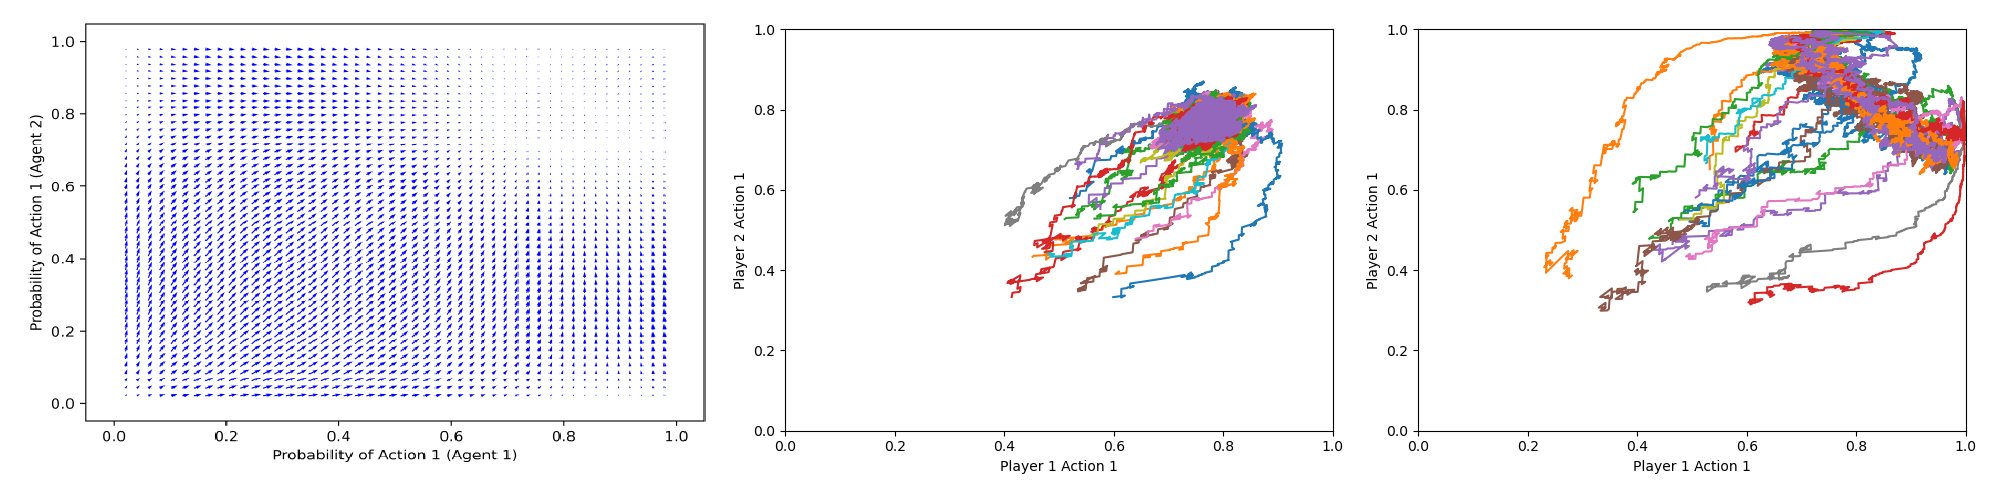
\includegraphics[width = \linewidth]{Figures/Gamma Var.png}
    \caption{Analysis of (\ref{eqn::EOM}) for the Prisoner's Dilemma Game. (Left) Vector field predicted by the continuous time model (\ref{eqn::EOM}). (Middle) Trajectories of action probabilities followed by Q-Learning agents trained on the iterated game with the parameters $\tau = 1$, $\alpha = 0.01$, $\gamma = 0.1$. (Right) Trajectories followed by agents with $\gamma = 0.75$.}
    \label{fig:Gamma Var}
\end{figure}

We then write the dynamics presented in \cite{Tuyls2006AnGames} in a general $p$-player game. This yields the expression
%
\begin{eqnarray}
%\begin{split}
    \label{eqn::pEOM}
    \frac{\dxmu{i}}{\xmu{i}{\mu}} & = & \alpha \tau ( \sum_{i_{-\mu}} \payoff{i}{\mu} \prod_{\kappa \neq \mu} \xmu{i}{\kappa} - \sum_{i_\mu i_{-\mu}} \xmu{i}{\mu} \payoff{i}{\mu} \prod_{\kappa \neq \mu} \xmu{i}{\kappa} ) + \alpha \sum_{j_\mu \in -i_\mu} \xmu{j}{\mu} ln \frac{\xmu{j}{\mu}}{\xmu{i}{\mu}},
%\end{split}
\end{eqnarray}

in which player $\mu$
chooses action $i_{\mu}$ from its strategy space $\mathcal{A}$ at time
$t$ with probability $\xmu{i}{\mu}$ and receives a reward
$\payoff{i}{\mu}$ from its payoff matrix $P^\mu$ depending on its own
action and the actions of all other agents $i_{-\mu}$, where $i_{-\mu}$ denotes the set $\{ i_\kappa : \kappa \in \{1, 2,
\ldots , p\} \setminus \{\mu\} \}$ and $-i_{\mu}$ denotes the set
$\mathcal{A} \setminus {i_\mu}$.

\subsection{Rescaling of Variables}

Our next port of call is to rescale the action probabilities and payoff elements. The rationale for this is as follows. The action probabilities, by definition, must satisfy the condition $\sum_{i_\mu} \xmu{i}{\mu} = 1$ and therefore $\xmu{i}{\mu}$ are of order $1/N$. The payoff elements (before scaling) are assumed to be drawn from a multivariate gaussian of mean zero and covariance
%
\begin{eqnarray}
\label{eqn::Payoffs}
%    \begin{split}
        \mathbb{E}\left [ \payoff{i}{\mu} \payoff{i}{\nu} \right] & = & \begin{cases}
        1 &  \text{ if } \nu = \mu \\
        \frac{\Gamma}{(p-1)} & \text{ otherwise. }
        \end{cases}
%    \end{split}
\end{eqnarray}

Therefore, the payoff elements are independent of $N$. As such, the expected payoff (i.e., the reward) that an agent receives, which is given by the term $\sum_{i_{-\mu}} \payoff{i}{\mu} \prod_{\kappa \neq \mu} \xmu{i}{\kappa}$, is of variance $1/N^{p-1}$. The standard deviation of this reward is therefore of order $1/\sqrt{N^{p-1}}$. As $N$ increases, and we shall be taking the limit $N \rightarrow \infty$, the expected payoffs will converge towards the same value and so appreciable steps in the Q-values will no longer be taken. To counteract this, the action probabilities and payoff elements are scaled as

\begin{eqnarray*}
%    \begin{split}
        \payoff{i}{\mu} & = & \tpayoff{i}{\mu} \sqrt{N^{p-1}}\\
        \xmu{i}{\mu} & = & \frac{\txmu{i}{\mu}}{N} 
%    \end{split}
\end{eqnarray*}

We also introduce the scaled parameters
\begin{eqnarray*}
%    \begin{split}
        \talpha & = & \frac{\alpha}{N} \\
        \ttau & = & N^{-(p-1)/2} \tau \\
        \htau & = & N^{-p/2} \tau
%    \end{split}
\end{eqnarray*}

which yields the scaled equation
%
\begin{eqnarray}
%\begin{split}
    \label{eqn::scaledEOM}
    \frac{\dtxmu{i}{\mu}}{\txmu{i}{\mu}} & = & \alpha \ttau \left ( \sum_{i_{-\mu}} \tpayoff{i}{\mu} \prod_{\kappa \neq \mu} \txmu{i}{\kappa} \right ) - \alpha \htau \left ( \frac{1}{\sqrt{N}} \sum_{i_\mu i_{-\mu}} \txmu{i}{\mu} \tpayoff{i}{\mu} \prod_{\kappa \neq \mu} \txmu{i}{\kappa} \right ) + \talpha \sum_{j_\mu \in -i_\mu} \txmu{j}{\mu} ln \frac{\txmu{j}{\mu}}{\txmu{i}{\mu}}
%\end{split}
\end{eqnarray}



The factor $\frac{1}{\sqrt{N}}$ is required in the derivation of the \textit{effective dynamics} and will become clear after taking the
expectation of the generating functional in the following section. Henceforth, we shall
not write the tildes on the action probabilities and payoffs. We shall also
abbreviate the final term as
%
	\begin{eqnarray*}
		\rho^{\mu}_{i}(t) & = & \sum_{j_\mu \in -i_\mu} \xmu{j}{\mu} ln \frac{\xmu{j}{\mu}}{\xmu{i}{\mu}}
	\end{eqnarray*}


\subsection{Generating Functional} % (fold)

The generating functional allows us to take a path integral over all possible realisations of
learning \cite{Mezard1986}. This is given as
%
\begin{equation}
	Z = \int D[\Vec{x}] \prod_i \delta(\textit{equation of motion}_i) exp(i
	\int dt[x_i(t) \psi_i(t)]), 
\end{equation}
%
where the equations of motion are the Lagrange equations of motion given in (\ref{eqn::scaledEOM}) and
the fields $\Vec{\psi_i(t)}$ and $\Vec{\phi_i(t)}$ will be set to zero at the end of the
calculation. $\delta$ denotes the Dirac delta function. We write this expression in its Fourier
representation which, after substituting (\ref{eqn::scaledEOM}) yields	
	%
\begin{equation}
	\begin{split}
\label{eqn::generatingfunctional}
	Z(\Vec{\psi}) = \int D[\Vec{x}, \Vec{\hat{x}}] exp(i \sum_{i, \mu} \int dt[\hxmu{i}  \{  \eom  -h_i^\mu (t) \} ) 
	\times exp(i \sum_{i, \mu}
	\int dt[\xmu{i} \psi^\mu_i(t)]),
\end{split}
\end{equation}
	
where the $\hxmu{i}$ indicates the Fourier transform of $\xmu{i}{\mu}$ and $h_i^\mu (t)$ denotes a perturbative field which too shall be set to zero. In order to determine the \textit{effective dynamics}, which gives the behaviour of an individual strategy component averaged over all payoff realisations, we will need to perform the averaging over $\payoff{i}{\mu}$. To do this, we first isolate the terms which contain $\payoff{i}{\mu}$.
	
\begin{equation}
	\begin{split}
	Z(\Vec{\psi}) = \int D[\Vec{x}, \Vec{\hat{x}}] exp \left( i \sum_{i, \mu} \int dt \left[ \hxmu{i} (\frac{\dxmu{i}}{\xmu{i}{\mu}} - \talpha \rho_i^\mu (t) - h_i^\mu (t)) \right] \right) \\
	\times exp \left(-i \alpha \ttau \sum_{i, \mu} \int dt \left [\hxmu{i} \left ( \sum_{i_{-\mu}} \payoff{i}{\mu} \prod_{\kappa \neq \mu} \xmu{i}{\kappa} \right ) \right] \right) \\
    \times exp(-i \alpha \ttau \sum_{i, \mu} \int dt [\hxmu{i} \left ( \sum_{i_\mu, i_{-\mu}} \xmu{i}{\mu} \payoff{i}{\mu} \prod_{\kappa \neq \mu} \xmu{i}{\kappa} \right )])) 
	\times exp(i \sum_{i, \mu}
	\int dt[\xmu{i} \psi^\mu_i(t)])
\end{split}
\end{equation}


We relabel $\hxmu{i}$ in the third exponential to $\hxmu{j}$ to distinguish it from $\xmu{i}{\mu}$. This is possible since $j_\mu$ is summed over.
%
\begin{equation}
	\begin{split}
	Z(\Vec{\psi}) = \int D[\Vec{x}, \Vec{\hat{x}}] exp \left( i \sum_{i, \mu} \int dt \left[ \hxmu{i} (\frac{\dxmu{i}}{\xmu{i}{\mu}} - \talpha \rho_i^\mu (t) - h_i^\mu (t)) \right] \right) \\
	\times exp \left(-i \alpha \ttau \sum_{\mu} \sum_{i_\mu, i_{-\mu}} \int dt \left [\hxmu{i} \payoff{i}{\mu} \prod_{\kappa \neq \mu} \xmu{i}{\kappa} \right] \right) \\
    \times exp \left(-i \alpha \ttau \sum_{\mu} \sum_{j_\mu, i_\mu, i_{-\mu}} \int dt \left[\hxmu{j}  \xmu{i}{\mu} \payoff{i}{\mu} \prod_{\kappa \neq \mu} \xmu{i}{\kappa} \right] \right)
	\times exp(i \sum_{i, \mu}
	\int dt[\xmu{i} \psi^\mu_i(t)])
\end{split}
\end{equation}

Having isolated the terms containing the payoff elements into their own exponentials, we are able, finally, to average over the possible realisations. In order to do this, we focus only on the exponentials which contain those elements, defining
%
\begin{subequations}
\begin{align}
    \mathbb{E}[Q_1] = \prod_{\mu, i_\mu, i_{-\mu}} \mathbb{E} \left[exp(-i \alpha \ttau \int dt \hxmu{i} \payoff{i}{\mu} \prod_{\kappa \neq \mu} \xmu{i}{\kappa}) \right] \\
    \mathbb{E}[Q_2] = \prod_{\mu, j_\mu, i_\mu, i_{-\mu}} \mathbb{E} \left[exp(i \frac{\alpha \htau}{\sqrt{N}} \int dt \hxmu{j} \xmu{i}{\mu} \payoff{i}{\mu} \prod_{\kappa \neq \mu} \xmu{i}{\kappa}) \right]
\end{align}
\end{subequations}

\subsubsection{Expectation of $Q_1$}

We first write $Q_1$ as 
%
\begin{eqnarray*}
    Q_1 & = & \prod_{ij} exp(\Vec{b} \cdot \Vec{z}),
\end{eqnarray*}
%
where
%
\begin{eqnarray*}
%    \begin{split}
       b & := & [ -i \alpha \ttau \int dt \hxmu{i} \prod_{\kappa \neq \mu} \xmu{i}{\kappa} ]^T 
%    \end{split}
\end{eqnarray*}
%
is a vector which contains all of the permutations of the products $\hxmu{i} \prod_{\kappa \neq \mu} \xmu{i}{\kappa}$ and

\begin{eqnarray*}
%    \begin{split}
       z & := & [ \payoff{i}{\mu} ]^T, 
%    \end{split}
\end{eqnarray*}
%
is a vector containing all of the payoff elements corresponding to the products in $b$. We then apply the exponential identity (whose proof is given in \cite{ZinnJustin2009})
%
\begin{eqnarray}
	\label{eqn::expectationIdentity}
		\int dz [e^{-A_2(z) + \Vec{b} \cdot \Vec{z}}] & = & (2 \pi)^{k/2} (det(A))^{-1/2} e^{\omega(b)},
	\end{eqnarray}
%
where
%
\begin{eqnarray*}
%	\begin{split}
		A_2(z) & = & 1/2 \sum_{ij} z_i A_{ij} z_j \\
		\omega_2(z) &  = & 1/2 \sum_{ij} b_i (A)^{-1}_{ij} b_j\\
%	\end{split}
%\end{equation*}
%
%and
%
%\begin{eqnarray*}
%    \begin{split}
       A  & = & \Sigma^{-1} \\
       \Sigma_{ij} & = & Cov[z_i, z_j].
%    \end{split}
\end{eqnarray*}

We recall that the scaled system has payoffs chosen so that
%
\begin{eqnarray}
\label{eqn::Payoffs}
%    \begin{split}
        \mathbb{E} \left[ \payoff{i}{\mu} \payoff{i}{\nu} \right] & = & \begin{cases}
        \frac{1}{\sqrt{N^{p-1}}}  & \text{ if } \nu = \mu \\
        \frac{\Gamma}{(p-1)\sqrt{N^{p-1}}} & \text{ otherwise. }
        \end{cases}
%    \end{split}
\end{eqnarray}

Applying the identity (\ref{eqn::expectationIdentity}) to $Q_1$ gives

\begin{eqnarray}
%\begin{split}
        \mathbb{E}[Q_1] & = exp & \left(  -\frac{\alpha^2 \ttau^2}{2 N^{p-1}} \sum_{i_\mu} \sum_\mu \int dt dt' \hxmu{i} \hxmudash{i} \prod_{\kappa \neq \mu} \xmu{i}{\mu} \prod_{\lambda \neq \mu} \xmudash{i}{\lambda} \right. \\
       & & \left. + \Gamma \sum_{\nu \neq \mu} \int dt dt' \hxmu{i} \hxnudash{i} \prod_{\kappa \neq \mu} \xmu{i}{\kappa} \prod_{\lambda \neq \nu} \xmudash{i}{\lambda}\right)
%\end{split}
\end{eqnarray}

\subsubsection{Expectation of $Q_2$}

We take a similar approach to that of $Q_1$ by defining
%
\begin{eqnarray*}
%    \begin{split}
       b & := & [\ldots i \alpha \htau \int dt \hxmu{j} \xmu{i}{\mu} \prod_{\kappa \neq \mu} \xmu{i}{\kappa} \ldots]^T \\
       z & := & [\ldots \payoff{i}{\mu} \ldots]^T, 
%    \end{split}
\end{eqnarray*}
%
in which $\ldots$ indicates that the entries are parameterised with respect to $\mu$ and then follow the same procedure to arrive at
%
\begin{eqnarray}
%\begin{split}
        \mathbb{E}[Q_2] & = exp & 
        \left(-\frac{\alpha^2 \htau^2}{2 N^{p}} \sum_{i_\mu} \sum_\mu \int dt dt' \hxmu{j} \xmu{i}{\mu} \hxmudash{j} \xmudash{i}{\mu} \prod_{\kappa \neq \mu} \xmu{i}{\mu} \prod_{\lambda \neq \mu} \xmudash{i}{\lambda} \right.\\
       & & \left. + \Gamma \sum_{\nu \neq \mu} \int dt dt' \hxmu{j} \hxnudash{j} \xmu{i}{\mu} \xmudash{i}{\nu} \prod_{\kappa \neq \mu} \xmu{i}{\kappa} \prod_{\lambda \neq \nu} \xmudash{i}{\lambda}\right).
%\end{split}
\end{eqnarray}

Next, we define the correlation functions
%
\begin{eqnarray*}
%    \begin{split}
       C^\mu (t, t') & := & N^{-1} \sum_{i} \xmu{i}{\mu} \xmudash{i}{\mu} \\
       L^\mu (t, t') & := & N^{-1} \sum_{i} \hxmu{i} \hxmudash{i} \\
       K^\mu (t, t') & := & N^{-1} \sum_{i} \xmu{i}{\mu} \hxmudash{i} \\
       A^{\mu, \nu} (t, t') & := & N^{-1} \sum_{i} \hxmu{i} \hxnudash{i},
%    \end{split}
\end{eqnarray*}
%
which allows us to rewrite the expectations as
%
\begin{equation}
\begin{split}
        \mathbb{E}[Q] = exp \left(- \frac{\alpha^2 \ttau ^2}{2} N \sum_{\mu} \Big [ \int dt dt' L^\mu(t, t') \prod_{\kappa \neq \mu} C^\kappa (t, t') +  \Gamma \sum_{\nu \neq \mu} K^\mu (t, t') K^\nu (t, t') \prod_{\kappa \not\in \{\mu, \nu\}} C^\kappa (t, t') \Big ] \right) \times \\
        exp \left(- \frac{\alpha^2 \htau ^2}{2} N \sum_{\mu} \Big [ \int dt dt' L^\mu(t, t') C^\mu (t, t') \prod_{\kappa \neq \mu} C^\kappa (t, t') +  \Gamma \sum_{\nu \neq \mu} A^{\mu \nu} (t, t') C^\nu (t, t') C^\mu (t, t') \prod_{\kappa \not\in \{\mu, \nu\}} C^\kappa (t, t') \Big ] \right)
\end{split}
\end{equation}

To introduce these correlation functions into the integral, we rely on the use of their Dirac delta functions in its Fourier transform, for example

\begin{equation}
    1 = \int D[C^\mu (t, t') \hat{C}^\mu (t, t')] \text{ } exp(iN \int dt dt' \text{ } \hat{C}^\mu (t, t') (C^\mu (t, t')) - N^{-1} \sum_{i} \xmu{i}{\mu} \xmudash{i}{\mu})
\end{equation}

\subsection{The Effective Dynamics}

Having performed the expectation of the variables $\payoff{i}{\mu}$ in the generating functional, we can now substitute (\ref{eqn::generatingfunctional}) to yield
%
\begin{equation}
    \label{eqn::averagedgf}
    \mathbb{E}[Z(\Vec{\psi})] = \int D[C, \hat{C}, L, \hat{L}, K, \hat{K}, A, \hat{A}] \text{ } exp(N (\Psi + \Phi + \Omega + \mathcal{O}(N^{-1}))),
\end{equation}
%
where
%
\small{
\begin{equation}
    \begin{split}
         \Psi = i \sum_\mu \int dt dt' \left[ C^\mu (t, t') \hat{C}^\mu (t, t') + L^\mu (t, t') \hat{L}^\mu (t, t') + K^\mu (t, t') \hat{K}^\mu (t, t') + \sum_{\nu \neq \mu} A^{\mu ]\nu} (t, t') \hat{A}^{\mu \nu} (t, t')]\right] \\
         \Phi = - \frac{\alpha^2 \ttau ^2}{2} N \sum_{\mu} \Big [ \int dt dt' L^\mu(t, t') \prod_{\kappa \neq \mu} C^\kappa (t, t') +  \Gamma \sum_{\nu \neq \mu} K^\mu (t, t') K^\nu (t, t') \prod_{\kappa \not\in \{\mu, \nu\}} C^\kappa (t, t') \Big ] \\
        - \frac{\alpha^2 \htau ^2}{2} N \sum_{\mu} \Big [ \int dt dt' L^\mu(t, t') C^\mu (t, t') \prod_{\kappa \neq \mu} C^\kappa (t, t') +  \Gamma \sum_{\nu \neq \mu} A^{\mu \nu} (t, t') C^\nu (t, t') C^\mu (t, t') \prod_{\kappa \not\in \{\mu, \nu\}} C^\kappa (t, t') \Big ] \\
         \Omega = N^{-1} \sum_{\mu, i_\mu} ln \Big \{ \int D[\xmu{i}{\mu}, \hxmu{i}] p_{i, 0}^\mu exp \left(i \int dt \xmu{i}{\mu} \psi_{i_\mu}^\mu \right) \times exp \left(i\int dt \left[ \hxmu{i} (\frac{\dxmu{i}}{\xmu{i}{\mu}} - \talpha \rho_i^\mu (t) - h_i^\mu (t)) \right] \right) \times \\ exp \left(-i \int dt dt' \left[\hat{C}^\mu (t, t') \xmu{i}{\mu} \xmudash{i}{\mu} + \hat{L}^\mu (t, t') )\hxmu{i} \hxmudash{i} + \hat{K}^\mu (t, t') )\xmu{i}{\mu} \hxmudash{i} + \sum_{\nu \neq \mu} \hat{A}^{\mu \nu} (t, t') \hxmu{i} \hxnudash{i} \right]  \right)  \Big \}.
    \end{split}
\end{equation}
}
Here, $p_{i, 0}^\mu$ denotes the initial distribution which the action is drawn from. It is important to note here that all of the information regarding the dynamics of the agent is included within $\Omega$, in the sense that the integral over the strategy components $x$ are contained within this expression. 

\subsection{Saddle Point Integration}

We now wish to reduce the integral (\ref{eqn::averagedgf}) through the use of the saddle point method of integration. In this method, we take the limit $N \rightarrow \infty$ so that the area under the curve of (\ref{eqn::averagedgf}) is dominated by the maxima of the term $(\Psi + \Phi + \Omega + \mathcal{O}(N^{-1}))$. Therefore, we first find the maxima of this term with respect to the integral variables $[C, \hat{C}, L, \hat{L}, K, \hat{K}, A, \hat{A}]$. This yields

\begin{eqnarray}
\frac{\partial f}{\partial \hat{C}^\mu} = 0  & \implies & C^\mu (t, t') =  - \lim_{N \rightarrow \infty} N^{-1} \sum_i \mathbb{E}[\xmu{i}{\mu} \xmudash{i}{\mu}]_{\Omega}  = - \lim_{N \rightarrow \infty} N^{-1} \sum_i \frac{\partial^2 \mathbb{E}[Z(\Vec{\psi})]}{\delta \psi_{i_\mu}^\mu (t) \psi_{i_\mu}^\mu (t')} \Big \rvert_{\Vec{\psi} = \Vec{h} = 0} \\
\frac{\partial f}{\partial \hat{L}^\mu} = 0  & \implies & L^\mu (t, t') =  - \lim_{N \rightarrow \infty} N^{-1} \sum_i \mathbb{E}[\hxmu{i} \hxmudash{i}]_{\Omega}  = - \lim_{N \rightarrow \infty} N^{-1} \sum_i \frac{\partial^2 \mathbb{E}[Z(\Vec{\psi})]}{\delta h_{i_\mu}^\mu (t) h_{i_\mu}^\mu (t')} \Big \rvert_{\Vec{\psi} = \Vec{h} = 0} \\
\frac{\partial f}{\partial \hat{K}^\mu} = 0  & \implies & K^\mu (t, t') =  - \lim_{N \rightarrow \infty} N^{-1} \sum_i \mathbb{E}[\xmu{i}{\mu} \hxmudash{i}]_{\Omega}  = - \lim_{N \rightarrow \infty} N^{-1} \sum_i \frac{\partial^2 \mathbb{E}[Z(\Vec{\psi})]}{\delta \psi_{i_\mu}^\mu (t) h_{i_\mu}^\mu (t')} \Big \rvert_{\Vec{\psi} = \Vec{h} = 0} \\
\frac{\partial f}{\partial \hat{A}^{\mu \nu}} = 0  & \implies & A^{\mu \nu} (t, t') =  - \lim_{N \rightarrow \infty} N^{-1} \sum_i \mathbb{E}[\hxmu{i} \hxnudash{i}]_{\Omega}  = - \lim_{N \rightarrow \infty} N^{-1} \sum_i \frac{\partial^2 \mathbb{E}[Z(\Vec{\psi})]}{\delta h_{i_\mu}^\mu (t) h_{i_\nu}^\nu (t')} \Big \rvert_{\Vec{\psi} = \Vec{h} = 0},
\end{eqnarray}
%
where $\mathbb{E}[ \cdot ]_\Omega$ denotes an expectation to be taken over $\Omega$. The interested reader may consult \cite{Coolen2005} for details on how such an expectation may be formulated. However, for our purposes, the details are not required. What it is important to note, however, is that by normalisation of the generating functional it was required that $Z(\Vec{\psi = 0}) = 1$ for any choice of $h$. Therefore, the $Z(\Vec{\psi})$ is constant in $h$ and therefore we have that $L^\mu (t, t') = 0$ and $A^{\mu \nu} = 0$ for any $t, t'$. In addition, we know that past values of $\xmu{i}{\mu}$ cannot be affected by future values and so we have that $K^\mu(t, t') = 0$ for $t' > t$ and so $K^\mu(t, t') K^\mu(t', t) = 0$.

Continuing the extrema analysis we have
%
\begin{eqnarray}
\frac{\partial f}{\partial C^\mu} = 0  & \implies & i \hat{C}^\mu (t, t') =  0 \\
\frac{\partial f}{\partial L^\mu} = 0  & \implies & i \hat{L}^\mu (t, t') = \frac{\alpha^2 \ttau ^2}{2} \prod_{\kappa \neq \mu} C^\kappa (t, t') + \frac{\alpha^2 \htau ^2}{2} C^\mu (t, t') \prod_{\kappa \neq \mu} C^\kappa (t, t') \\
\frac{\partial f}{\partial K^\mu} = 0 & \implies & i \hat{K}^\mu (t, t') = \alpha^2 \ttau ^2 \Gamma \sum_{\nu \neq \mu} K^\nu (t, t') \prod_{\kappa \not\in \{\mu, \nu\}} C^\kappa (t, t') \\
\frac{\partial f}{\partial A^{\mu \nu}} = 0 & \implies & i \hat{A}^{\mu \nu} (t, t') = \frac{\alpha^2 \htau ^2}{2} \Gamma \sum_{\nu \neq \mu} (t, t') C^\nu (t, t') C^\mu (t, t') \prod_{\kappa \not\in \{\mu, \nu\}} C^\kappa (t, t'),
\end{eqnarray}
%
where the first equality holds since in $\Omega$, $C^\mu (t, t')$ always appears in a product with $L^\mu (t, t')$, $A^{\mu \nu}$ or $K^\mu(t, t') K^\mu(t', t)$, which we have already established to be 0. By substituting these expressions back into (\ref{eqn::averagedgf}), we immediately get that $\Psi + \Phi = 0$ since each of the terms will contain one of the above terms which we found to be 0. For $\Omega$, we get

\begin{equation}
\begin{split}
        \Omega = N^{-1} \sum_{\mu, i_\mu} ln \Big \{ \int D[\xmu{i}{\mu}, \hxmu{i}] p_{i, 0}^\mu exp (i \int dt \xmu{i}{\mu} \psi_{i_\mu}^\mu) \times exp \left(i \int dt \left[ \hxmu{i} (\frac{\dxmu{i}}{\xmu{i}{\mu}} - \talpha \rho_i^\mu (t) - h_i^\mu (t)) \right] \right) \times \\ exp \Bigg(-i \int dt dt' \left[\frac{\alpha^2 \ttau ^2}{2} \prod_{\kappa \neq \mu} C^\kappa (t, t') \hxmu{i} \hxmudash{i} + \frac{\alpha^2 \htau ^2}{2} C^\mu (t, t') \prod_{\kappa \neq \mu} C^\kappa (t, t') \hxmu{i} \hxmudash{i} + \\ \alpha^2 \ttau ^2 \Gamma \sum_{\nu \neq \mu} K^\nu (t, t') \prod_{\kappa \not\in \{\mu, \nu\}} C^\kappa (t, t') \xmu{i}{\mu} \hxmudash{i} + \\ \frac{\alpha^2 \htau ^2}{2} \Gamma \sum_{\nu \neq \mu} (t, t') C^\nu (t, t') C^\mu (t, t') \prod_{\kappa \not\in \{\mu, \nu\}} C^\kappa (t, t') \hxmu{i} \hxnudash{i} \right] \Bigg)   \Big \}.
\end{split}
\end{equation}

We make the assumption that all strategy components for all agents are drawn from the same initial distribution $p_0$, are under the influence of the same perturbative field $h(t)$ and also finally set the generating field $\psi = 0$, we are able to drop the distinction between agents and their action probabilities. Instead, we regard that all actions are independent and identically distributed (i.i.d). This is a strong assumption, but is required to ensure that the strategy components are all positive and real-valued (which is required for a probability). This gives $\Omega$ as
%
\begin{eqnarray}
%\begin{split}
        \Omega & = & pln \Big \{ \int D[x, \hat{x}] p_{0} exp \left(i \int dt \left[ \hat{x}(t) (\frac{\dot{x}}{x} - \talpha \rho (t) - h(t)) \right] \right) \times \nonumber \\ & & exp \Bigg(-i \int dt dt' \Big[\frac{\alpha^2 \ttau ^2}{2} C^{(p-1)} (t, t') \hat{x}(t) \hat{x}(t') + \frac{\alpha^2 \htau ^2}{2} C^{(p-1)} (t, t') \hat{x}(t) \hat{x}(t') + \nonumber  \\ & & \alpha^2 \ttau ^2 \Gamma (p-1) i G(t, t') C^{(p-1)} (t, t') x(t) \hat{x}(t') +  \frac{\alpha^2 \htau ^2}{2} \Gamma (p-1) A(t, t') C^{(p-1)} (t, t') \hat{x}(t) \hat{x}(t') \Big] \Bigg) \Big \},
%\end{split}
\end{eqnarray}
%
where $G(t, t') = -iK(t, t')$. 

We note here that since we have dropped the distinction between players, the term $A^{\mu, \nu}$ which coupled the actions of players together is now no longer meaningful and can be identified with the uncoupled term $L(t, t')$. This identification is the strongest of our assumptions and results in a deviation from the initial, coupled, nature of the dynamics (\ref{eqn::pEOM}). However, as mentioned, it is required to yield a physically viable expression for action probabilities (i.e., positive real valued). In addition, since each strategy component is independent, the expression for $\Omega$ can be decomposed to yield an individual \textit{effective generating functional} for each component given as

\begin{eqnarray}
\label{eqn::zeff}
%\begin{split}
        Z_{eff} & = & \int D[x, \hat{x}] p_{0} exp \left(i \int dt \left[ \hat{x}(t) (\frac{\dot{x}}{x} - \talpha \rho (t) - h(t)) \right] \right) \times \nonumber \\
        & & exp \Bigg(-i \int dt dt' \Big[\alpha^2 \ttau ^2 C^{(p-1)} (t, t') \hat{x}(t) \hat{x}(t') + \alpha^2 \htau ^2 C^{(p-1)} (t, t') \hat{x}(t) \hat{x}(t') + \nonumber \\
        & & i \alpha^2 \ttau ^2 \Gamma  G(t, t') C^{(p-1)} (t, t') x(t) \hat{x}(t') \Big] \Bigg).
%\end{split}
\end{eqnarray}

We notice that (\ref{eqn::zeff}) is exactly the form of the generating functional for the dynamics
%
\begin{equation}
    \label{eqn::EffectiveDynamics}
    \begin{split}
            \frac{1}{x(t)} \frac{d}{dt} x(t) = \alpha^2 \ttau^2 \Gamma \int dt' \left [G(t, t')C^{p - 2}(t, t') x(t') \right ] + \sqrt{2} \alpha \ttau \eta_1(t) + \sqrt{2} \alpha \htau \eta_0(t) + \talpha \rho(t), 
    \end{split}
\end{equation}
%
where
%
\begin{eqnarray*}
%    \begin{split}
        C(t, t') & = & \mathbb{E}[x(t) x(t')] \\
        \mathbb{E}[\eta_1(t)] & = & 1, \text{ \space } \mathbb{E}[\eta_1(t) \eta_1(t')]  =  C^{p-1}(t, t') \\
        \mathbb{E}[\eta_0(t)] & = & 1, \text{ \space } \mathbb{E}[\eta_0(t) \eta_0(t')] = C^{p}(t, t') \\
        G(t, t') & = & \mathbb{E}\left [ \frac{\delta x(t)}{ \delta \eta_1(t')} \right].
%    \end{split}
\end{eqnarray*}

We therefore call (\ref{eqn::EffectiveDynamics}) the \textit{effective dynamics}. This gives an approximate expression for the expected behaviour of a strategy component averaged over all possible realisations of the payoff matrix. It is on this system that we will perform a stability analysis.

\section{Fixed Points of the System}

Before we can analyse the stability of a fixed point, we first need to establish that the fixed point exists for the system. At such a point $\dot{x}(t) = 0$. Furthermore, since there is no fluctuation of $x(t)$ with respect to time, the term $C(t, t')$ is constant and $G(t, t') \approx G(t - t')$. As $\eta_0, \eta_1$ are also both stationary at the fixed point, we rewrite $\eta_1$ as $q^{(p-1)/2}z$ where $q = \mathbb{E}[\xfixed^2]$ and $z$ is drawn from the standard normal distribution (mean 0, variance 1). This gives $\eta_0 = q^{p/2}z^{p/p-1}$. To ensure, once again, that $x(t)$ remains real valued, we must avoid fractional powers in $z$, which itself can be negative valued. Therefore, we make the assumption that $p$ is large enough so that $p \approx p-1$. Then $\eta_0 \approx q^{p-1/2}z = \eta_1$. With all of the above considered, (\ref{eqn::EffectiveDynamics}) reduces to the fixed point equation

\begin{eqnarray}
%    \begin{split}
    0 = \xfixed [ \alpha^2 \ttau^2 \Gamma \xfixed q^{p-2} \chi 
       + \sqrt{2} q^{(p-1)/2}z (\alpha \ttau  + \alpha \htau) + \talpha \rho]
    \label{eqn::fixed_point}
%    \end{split}
\end{eqnarray}
%
where $\chi = \int G(t-t') dt $. Now, we have two possible choices for the fixed point: either $\xfixed$ is zero or $\xfixed$ is given by the expression in the squared brackets. The former is never achieved in practice; an agent will not assign an action to have exactly zero probability. Therefore, we only consider the latter term with $\xfixed$ given as

\begin{equation}
    \xfixed = \frac{- \sqrt{2} q^{(p-1)/2}z (\alpha \ttau  + \alpha \htau) + \talpha \rho}{\alpha^2 \ttau^2 \Gamma  q^{p-2} \chi}.
\end{equation}

Due to causality, we have that $\chi > 0$ for $\Gamma < 0$ \cite{Opper1992, Galla2013}. It is therefore in this region that the existence of a unique, positive solution to (\ref{eqn::fixed_point}) can be understood, for the case that the numerator remains negative. However, for positive $\Gamma$ this relation does not necessarily hold and so the behaviour of the system for positive $\Gamma$ is not well understood. Therefore, we must restrict our analysis to $\Gamma \in [-1, 0]$.

Of course, the expression in the brackets of (\ref{eqn::fixed_point}) is not trivial to solve and so a Newton-Raphson root finding method was employed to approximate the value. The parameters $q, \chi, \rho$ are determined as
%
\begin{eqnarray*}
        1 & = & \frac{1}{\sqrt{2 \pi}} \int_{-\infty}^{\infty} \xfixed(z) exp(-\frac{z^2}{2}) dz \\ 
        q & = & \frac{1}{\sqrt{2 \pi}} \int_{-\infty}^{\infty} \xfixed(z)^2 exp(-\frac{z^2}{2}) dz \\ 
        \chi & = & \frac{1}{q^{n/2}}\frac{1}{\sqrt{2 \pi}} \int_{-\infty}^{\infty} \frac{\partial \xfixed (z)}{\partial z} exp(-\frac{z^2}{2}) dz\\
        \rho & = & \frac{1}{\sqrt{2 \pi}} \int_{-\infty}^{\infty} \xfixed(z') ln \frac{\xfixed(z')}{\xfixed(z)} dz'
\end{eqnarray*}

\section{Stability of the Effective Dynamics}

With the region $\Gamma < 0$ established and the fixed point examined, we now look at the behaviour of the effective dynamics in a neighbourhood of the fixed point. In particular, we would like to establish whether, if perturbed from the $\xfixed$, the system will diverge away (unstable) or converge to $\xfixed$ (stable). A similar question was considered by Opper and Diederich in \cite{Opper1992} and so we progress along the same lines. 

The dynamics are proposed to be perturbed by a
disturbance $\xi(t)$ which is drawn from a Gaussian of zero mean and
unit variance. The disturbance causes the values of $x(t)$ and
$\eta_0(t)$, $\eta_1(t)$ to deviate from their fixed point position
$\xfixed$, $\ezerof$, $\eonef$ by an amount $\xpert$, $\ezeropert$,
$\eonepert$. Rewriting the dynamics with all of these considerations yields
%
\begin{eqnarray}
 %   \begin{split}
            \frac{d}{dt} (\xfixed + \xpert(t)) & = & (\xfixed + \xpert(t)) \Big (\alpha^2 \ttau^2 \Gamma \int dt' \left [G(t, t')C^{p - 2}(t, t') (\xfixed + \xpert(t')) \right ]  \nonumber \\
            & & + \sqrt{2} \alpha \ttau (\eonef + \eonepert(t')) + \sqrt{2} \alpha \htau (\ezerof + \eonepert(t)) + \talpha \rho + \xi(t) \Big )
  %  \end{split}
\end{eqnarray}

In a neighbourhood of $\xfixed$, the linear terms would dominate and so we keep these, neglecting higher order terms. This yields
%
\begin{eqnarray}
%    \begin{split}
\frac{d}{dt} \xpert & = & (\xfixed + \xpert) [ \alpha^2 \ttau^2 \Gamma \xfixed \int dt' [ G(t, t')C^{p - 2}(t, t') ] \nonumber + \sqrt{2} \alpha \ttau \eonef + \sqrt{2} \alpha \htau \ezerof + \talpha \rho] \nonumber \\
& &  + \xfixed [\alpha^2 \ttau^2 \Gamma \int dt' [ G(t, t')C^{p - 2}(t, t') \xpertdash ] + \sqrt{2} \alpha \ttau \eonepert + \sqrt{2} \alpha \htau \ezeropert + \xi(t)]
\label{eqn::Linearised}
%    \end{split}
\end{eqnarray}

Now invoking the fixed point condition, we notice that the first square bracket in (\ref{eqn::Linearised}) equates to zero. Now, taking the Fourier transform of (\ref{eqn::Linearised}) gives

\begin{equation}
    \Big[ \frac{i \omega}{\xfixed} - \alpha^2 \ttau^2 \Gamma \tilde{H(\omega)} \Big] \tilde{X(\omega)} = \sqrt{2} \alpha \ttau \tilde{\eta_1 (\omega)} + \sqrt{2} \alpha \htau \tilde{\eta_0 (\omega)} + \tilde{\Xi(\omega)}
\end{equation}
%
where $H(t) = G(t, t')C^{(p-2)}(t, t')$. 

Using the self-consistency relation that $\mathbb{E}[|\eonef^2|] = (p-1)\mathbb{E}[|\xfixed^2|]^{(p-2)}\mathbb{E}[|\tilde{X}(\omega)^2|]$ and, once again, the estimate $\mathbb{E}[|\tilde{\eta_1 (\omega)}^2|] \approx \mathbb{E}[|\tilde{\eta_0 (\omega)}^2|]$ in the region where $p \approx p-1$ we have

\begin{eqnarray}
    \mathbb{E}\Big[| \frac{i \omega}{\xfixed} - \alpha^2 \ttau^2 \Gamma \tilde{H(\omega)}|^2 \Big] \mathbb{E}[|\tilde{X(\omega)}|^2] & = & \mathbb{E}[|\sqrt{2} \alpha \ttau \tilde{\eta_1 (\omega)} + \sqrt{2} \alpha \htau \tilde{\eta_0 (\omega)} + \tilde{\Xi(\omega)}|^2] \nonumber \\
    & = & 2 \alpha^2 \ttau^2 \mathbb{E}[|\tilde{X(\omega)}|^2] + 4 \alpha^2 \ttau \htau \mathbb{E}[|\tilde{X(\omega)}|^2] + 2 \alpha^2 \htau^2 \mathbb{E}[|\tilde{X(\omega)}|^2] + 1 \nonumber \\
    \mathbb{E}[|\tilde{X(\omega)}|^2] & = & \Big ( \mathbb{E}\Big[| \frac{i \omega}{\xfixed} - \alpha^2 \ttau^2 \Gamma \tilde{H(\omega)}|^2 \Big] - 2(\alpha \ttau + \alpha \htau)^2 \Big )^{-1}
\end{eqnarray}

As we wish to examine the long time behaviour of the system, we must consider the case $\omega \rightarrow 0$. By definition, we require that $\mathbb{E}[|\tilde{X(\omega)}|^2] > 0$ (as it is a square, and an absolute). Therefore, if we find, for a given choice of parameters, that $\mathbb{E}[|\tilde{X(\omega)}|^2]$ yields a negative value, then the fixed point analysis breaks down and we have the onset of instability. As such, our criteria for a stable fixed point becomes

\begin{equation}
    \label{eqn::Final}
    0 \leq \left [(\alpha^2 \ttau^2 \Gamma q^{p-2} \chi)^{2} - 2 (\alpha \ttau + \alpha \htau)^2 (p-1)q^{p-2} \right ]
\end{equation}

Finally, (\ref{eqn::Final}) is the expression whose predictions are analysed in \cite{MainPaper}. 

\section{Experimental Code}

The following code was used to produce all of the experimental figures shown in the main paper \cite{MainPaper}. This is written in Julia 1.5 and the dependencies are listed in the first cell. To generate any of the heatmaps, first change the values of the parameters $\alpha, \tau, \Gamma, p, N$ to the desired choice. Then run the subsequent cells up to `plotHeatmap(a)'. To generate the variance plots run both the `getVariance' function and the subsequent cell.

\subfile{pPlayerJulia.tex}

\bibliographystyle{acm} 
\bibliography{references}

\end{document}
